\documentclass[11pt,a4paper]{article}
%%%%%%%%%%%%%%%%%%%%%%%%%%%%%%%%%%%%%%%%%%%%%%%%%%%%%%%%%%%%%%%%%%%%%%%%%%%%%%%%%%%%%%%%%%%%%%%%%%%%
%% PACKAGES
%%
%%
%% EXTRAS
\usepackage[type={CC},modifier={by-nc-sa},version={3.0}]{doclicense}
%% LAYOUT
\usepackage[top=1cm,bottom=1cm,left=1cm,right=1cm]{geometry}
\usepackage{pdflscape}
\usepackage[final]{pdfpages}
\usepackage[myheadings]{fullpage}
\usepackage{enumerate}
\usepackage{parskip}
\usepackage{dashrule}
\usepackage{enumitem}
\usepackage{sectsty}
\usepackage{latexsym}
\usepackage{framed}
\usepackage{pbox}
%% TeX MACROS
\usepackage{ifdraft}
%% LANGUAGE
\usepackage[english]{babel}
%% TEXT & TYPESETS
\usepackage{fourier}
\usepackage{shadowtext}
\usepackage[utf8]{inputenc}
\usepackage[T1]{fontenc}
\usepackage[protrusion=true, expansion=true]{microtype}
\usepackage{textcomp}
\usepackage{soul}
\usepackage{lipsum}
\usepackage{blindtext}
%% GRAPHICS & FIGURES
\usepackage{graphicx}
\usepackage{float}
\usepackage{wrapfig}
\usepackage{rotating}
\usepackage{tikz}
\usepackage{tikzpagenodes}
\usepackage[font=small, labelfont=bf]{caption}
\usepackage{pgfgantt}
%% MATH & SCIENCE
\usepackage{amsmath}
\usepackage{bm}
\usepackage{amssymb}
\usepackage{marvosym}
\usepackage{mathpazo}
\usepackage{mathtools}
\usepackage{siunitx}
%% TABLES
\usepackage{tabularx}
\usepackage{longtable}
\usepackage{array}
\usepackage{makecell}
%% HEADER & FOOTER
\usepackage{totpages,fancyhdr}
\def\ORGTITLE  {Research Plan}
\def\ORGAUTHOR {DP@H$_2$O}
\pagestyle{fancy}
\fancyhf{}
\setlength\headheight{1cm}
\fancyhead[L]{\LARGE \ORGTITLE  }
\fancyhead[R]{\large \ORGAUTHOR }
\fancyfoot[C]{\small Page \thepage}
%% BIBLIOGRAPHY
\usepackage[round]{natbib}
\bibliographystyle{abbrvnat}
%% \bibliographystyle{ksfh_nat}
%% HYPERLINK
\usepackage{url}
\usepackage{booktabs}
\usepackage{hyperref}
\hypersetup{
  colorlinks=true,
  linktoc=all,
  linkcolor=blue,
  filecolor=magenta,
  urlcolor=cyan,
  citecolor=magenta
}
%% SPACING
\usepackage{setspace}
%%\doublespace % draft: double; final: single spacing
%% TITLE & TOC
\usepackage{titling}
\title{\textsc{Research Plan}}
\author{\href{mailto:daniel.atwater@utas.edu.au}{Daniel Patrick Atwater}}
\setcounter{secnumdepth}{1}
\setcounter{tocdepth}{1}
%% COLOUR
\usepackage{xcolor}
%%%%%%%%%%%%%%%%%%%%%%%%%%%%%%%%%%%%%%%%%%%%%%%%%%%%%%%%%%%%%%%%%%%%%%%%%%%%%%%%%%%%%%%%%%%%%%%%%%%%
%% DEFINITIONS & NEWCOMMANDS
\newcommand{\crule}[3][black]{\textcolor{#1}{\rule{#2}{#3}}}
\newcommand{\source}[1]{\caption*{\hfill Source: {#1}} }
\newcommand{\HRule}[1]{\rule{\linewidth}{#1}}
\newcommand{\latlonDec}[2]{$\ang{#1}$ \textbf{#2}}
\newcommand{\citationNeeded}{\textbf{}}
\newcommand{\htwoo}{H$_2$O}
\newcommand{\otwo}{O$_2$}
\newcommand{\cotwo}{CO$_2$}
\newcommand{\chfour}{CH$_4$}
\newcommand{\ntwo}{N$_2$}
\newcommand{\moc}{\textit{\textsc{moc}}} %Meridional Overturning Circulation
\newcommand{\nadw}{\textit{\textsc{nadw}}} %Meridional Overturning Circulation
\newcommand{\sip}{\textit{\textsc{sip}}} %Sea ice production
\newcommand{\dsw}{\textit{\textsc{{dsw}}}} %Dense Shelf Water
\newcommand{\aabw}{\textit{\textsc{{aabw}}}} %Antarctic Bottom Water
\newcommand{\asf}{\textit{\textsc{{asf}}}} %Antarctic Slope Front
\newcommand{\asc}{\textit{\textsc{{asc}}}} %Antarctic Slope Current
\newcommand{\acc}{\textit{\textsc{{acc}}}} %Antarctic Slope Current
\newcommand{\cdp}{\textit{\textsc{{cdp}}}} %Cape Darnley Polynya
\newcommand{\cdfi}{\textit{\textsc{{cdfi}}}}
\newcommand{\mc}{\textit{\textsc{{mc}}}} %Mawson Coast
\newcommand{\ais}{\textit{\textsc{{ais}}}} %Amery Ice Shelf
\newcommand{\fastice}{fast ice}
\newcommand{\Fastice}{Fast ice}
%\newcommand{\Lpolynya}{$\mathcal{L}$-polynya}
%\newcommand{\Tpolynya}{$\mathcal{T}$-polynya}
\newcommand{\wmo}{\href{https://public.wmo.int/en}{\uppercase{wmo}}}
\newcommand{\utas}{\href{https://utas.edu.au}{\textsc{UTas}}}
\newcommand{\aapp}{\href{https://aappartnership.org.au}{\uppercase{aapp}}}
\newcommand{\imas}{\href{https://www.imas.utas.edu.au}{\uppercase{imas}}}
\newcommand{\csiro}{\href{https://www.csiro.au/en/about/people/business-units/oceans-and-atmosphere}{\uppercase{csiro}}}
\newcommand{\bom}{\href{http://www.bom.gov.au}{\uppercase{bom}}}
\newcommand{\anu}{\href{http://www.anu.edu.au}{\uppercase{anu}}}
\newcommand{\primarysupervisor}{\href{mailto:alexander.fraser@utas.edu.au}{\textsc{Alex Fraser}}}
\newcommand{\primaryadvisor}{\href{mailto:paul.sandery@csiro.au}{\textsc{Paul Sandery}}}
\newcommand{\secondarysupervisor}{\href{mailto:will.hobbs@utas.edu.au}{\textsc{Will Hobbs}}}
%\newcommand{\tertiarysupervisor}{\href{mailto:phillip.reid@utas.edu.au}{\textsc{Phillip Reid}}}
%\newcommand{\tertiarysupervisor}{\href{mailto:kaight@bas.ac.uk}{\textsc{Kaitlin Naughten}}}
\newcommand{\quarternarysupervisor}{\href{mailto:wilma.huneke@anu.edu.au}{\textsc{Wilma Huneke}}}
\newcommand{\grc}{\href{mailto:maxim.nikurashin@utas.edu.au}{\textsc{Max Nikurashin}}}
%%%%%%%%%%%%%%%%%%%%%%%%%%%%%%%%%%%%%%%%%%%%%%%%%%%%%%%%%%%%%%%%%%%%%%%%%%%%%%%%%%%%%%%%%%%%%%%%%%%%
%% BEGIN DOCUMENT
\begin{document}
\maketitle
\begin{tikzpicture}[remember picture,overlay]
  \node[above right, inner sep=0pt] at (current page header area.south west)
       {\includegraphics[height=33pt]{/home/dpath2o/PHD/graphical/logos/AAPP-logo-H}};
       \node[above left, inner sep=0pt] at (current page header area.south east)
            {\includegraphics[height=33pt]{/home/dpath2o/PHD/graphical/logos/UniTas_IMAS_Primary_Pos_RGB-2048x1001}};
\end{tikzpicture}
\tableofcontents
\newpage
%%%%%%%%%%%%%%%%%%%%%%%%%%%%%%%%%%%%%%%%
\section*{Thesis Title}
\addcontentsline{toc}{section}{\protect\numberline{}Thesis Title}%
Prognostic landfast sea ice and quantification of the relationship with
Antarctic Bottom Water formation off the coast of Cape Darnley, East Antarctica.
\section*{Supervisors \& Advisors}
\addcontentsline{toc}{section}{\protect\numberline{}Supervisors \& Advisors}%
\begin{itemize}
\item \primarysupervisor~$\rightarrow$ Primary Supervisor $\rightarrow$ \aapp~\& \imas
%\item \primaryadvisor~$\rightarrow$ Research Advisor $\rightarrow$ \csiro
\item \secondarysupervisor~$\rightarrow$ Supervisor $\rightarrow$ \aapp~\& \imas
%\item \tertiarysupervisor~$\rightarrow$ Supervisor $\rightarrow$ \bom~\& \aapp
\item \quarternarysupervisor~$\rightarrow$ Supervisor $\rightarrow$ \anu
\item \grc~$\rightarrow$ Grduate Research Coordinator $\rightarrow$ \imas
\end{itemize}
%%%%%%%%%%%%%%%%%%%%%%%%%%%%%%%%%%%%%%%%
\section*{Background}
\addcontentsline{toc}{section}{\protect\numberline{}Background}%

The meridional overturning circulation (\moc) within the Earth's ocean basins is understood to play a significant contribution in regulating heat content of the climate, ventilating the deep ocean and \cotwo~uptake \citep{Orsi1999,Levitus2005,Bindoff2007,Purkey2010,Talley2013}. With overturning
time scales on the order of a millennia \citep{Johnson2008} understanding the
driving mechanisms of the \moc~has implications for the rates of change of key
parameters in Earth's climate: e.g. \cotwo~uptake rate, latent heat draw down,
and ventilation of the deep ocean \citep{Bindoff2007,Purkey2010}.

The conceptual model of the \moc~includes the tropical waters of the Atlantic flowing north via the Gulf Stream
and overturning at various locations in the north Atlantic due to baroclinic
instabilities, thus becoming North Atlantic Deep Water. At the other
end of planet, along the coast of Antarctica, a complex set
of seasonal events give rise to coastal processes that cause cold dense water
to form at the surface at key locations \citep{Orsi1999,Talley2013}. As the water
forms it is highly unstable and begins to sink flowing down the slopes of the
continental shelf, mixing with ambient waters in its descent, and in the process
becoming dense shelf water (\dsw) \citep{Orsi2001}.
%Both Ekman forced and baroclinic instabilities transport \citep{Rintoul2018}
This \dsw~flows across the Antarctic slope front, with some indication of mixing \citep{Mizuta2021,VanAchter2021,Rintoul2018}, and into the various abyssal plains (e.g. becoming Antarctic Bottom Water \textemdash \aabw)
\citep{Stewart2019}. This water mass fills the ocean basins of the Southern Hemisphere \citep{Johnson2008}, and is
identified as cold dense abyssal water originating from overturning coastal
waters around Antarctica \citep{Orsi1999}.

In this manner, \aabw~mass accounts for 30\textendash 40\% of global ocean
mass \citep{Johnson2008}. Its formation and controlling mechanisms are areas of contemporary research. In the effort to prognosticate furture climate, the current capability to constrain the climate's heat budget,
via global climate models, is dependent upon knowledge of these
controlling mechanisms of the deep ocean
\citep{Domingues2008,Murphy2009,Purkey2012,Durack2018}. At present, the
uncertainty in deep-ocean heat uptake has been shown to be a significant cause
of variation among climate models \citep{Boe2009,Durack2018}. While on the other hand, empirically, it also has been
shown that Earth's systems linked to the long-term water-phase-mass distribution
and surface temperature variations are accelerating
\citep{Murphy2009,IPCC2019SpecialReport}.

One specific uncertainty of the \moc~under investigation in this
work, is the rate at which \aabw~is formed via \dsw~formation. To investigate
this uncertainty I will be undertaking a series of simulations of a coupled
physical system (sea ice-ocean) over a region of East Antarctica in the vicinity
of the Mawson Coast, see \ref{fig:GEBCO_bathy}.

%%%%%%%%%%%%%%%%%%%%%%%%%%%%%%%%%%%%%%%%
\section*{Rationale}
\addcontentsline{toc}{section}{\protect\numberline{}Rationale}%

The region of East Antarctica under investigation here, is chosen due to its:
\begin{enumerate}
\item significance in \aabw~formation
  \citep{Williams2010,Ohshima2016,Tamura2016,Williams2016,Fraser2019,Aoki2020},
\item previous remote sensing, oceanographic a geographic studies (i.e. data availability)
  \citep{Meijers2010,Williams2010,Ohshima2013,Tamura2016,Fraser2019,Aoki2020,Smith2020},
  and
\item previous geophysical fluid modelling covering or adjacent to this region
  and investigating oceanographic results
  \citep{Galton-Fenzi2012,Nakayama2014,Liu2017,Kusahara2017a,Kusahara2017b,Naughten2018,VanAchter2021}.
\end{enumerate}

The distinction of the Mawson Coast, in this context, is its inclusion of the Cape Darnley Polynya
(\cdp). The \cdp~\citep{Meijers2010,Ohshima2013} is a coastal ocean polynya
(i.e. latent\textendash heat polynya) \citep{Massom1999,Tamura2008}. Some coastal ocean
polynyas are sources of \aabw~\citep{Massom1999,Maqueda2004,Tamura2008}. For
reasons of clarification, I will use the \cite{Barber2007} definition of
polynyas:
\begin{quote}
  Polynyas are persistent reoccurring regions of open water and/or thin ice,
  tens to tens of thousands of square kilometres in extent, that occur at
  locations where more consolidated and thicker ice cover would be
  climatologically expected.
\end{quote}
This defintion is derived, in part, from \cite{Smith1990} and requires a
further, modern qualification, and that is that polynyas are \textit{non-linear}
regions \citep{Massom1999} of open water and/or thin ice. The inverse of this
given by \cite{Smith1990} in their definition of oceanographic \textit{leads} as
\textit{linear} openings in sea ice differentiated by their absence of
re-occurrence at a particular geographic location. For completeness, it should
be added, that coastal ocean polynyas are distinctly different from open ocean
polynyas in that the former are associated with sea ice production (\sip),
salt-rejection and hence \dsw~formation
\citep{Massom1999,Maqueda2004,Tamura2008}. This is in contrast to open ocean
polynyas (i.e. sensible heat polynyas) that are not typically associated with
\sip, especially in the Southern Ocean. Categorically, it is the water mass
modification occurring in coastal polynyas of Antarctica which are a key driver of the \moc~\citep{Gawarkiewicz1995,Orsi1999,Galton-Fenzi2012,Sansiviero2017},
and particularly, of concern in this work, is that the \cdp~has been shown to
contribute 13\textendash 30\% of the total \aabw~mass \citep{Ohshima2013}.

Given the identification of the \cdp~as a significant contributor to \aabw, the
effort to determine its controlling factors has been pursued \citep{Nakayama2014,Liu2017}. \cite{Fraser2019}
have shown that the contribution, specifically the length of landfast ice (\fastice), termed Cape Darnley \fastice~(\cdfi) is the most corollary physical feature (measured by satellite) in relation to the size of \cdp. (Note, I
include here the `dagger' portion, defined by \cite{Fraser2019}, when
considering \cdfi). Beyond the physical importance of \fastice~with polynya
dynamics it should be further ascribed that their role within the environment as unique habitats
is critical and our knowledge is formative \citep{Trathan2011,Ainley2015}. It may also be worth mentioning here, that conceptually
differentiating \fastice~from other types of sea ice (e.g. pack
ice, floes, etc.), I do so inline with common practice via the World
Meteorological Definition (\wmo) definition \cite{WMOSeaIceNomenclature}:
\begin{quote}
  Sea ice which forms and remains fast along the coast, where it is attached to
  the shore, to an ice wall, to an ice front, between shoals or grounded
  icebergs. Vertical fluctuations may be observed during changes of sea-level.
  Fast ice may be formed in situ from sea water or by freezing of floating ice
  of any age to the shore, and it may extend a few metres or several hundred
  kilometres from the coast. Fast ice may be more than one year old and may then
  be prefixed with the appropriate age category (old, second-year, or multi-
  year).
\end{quote}

In many parts of the Antarctic continental shelf bathymetry favours the grounding of
icebergs \citep{Wesche2012}. The grounding of icebergs provides a linking/trapping/blocking
mechanism for sea ice to become fastened to the iceberg \citep{Massom2000,Fraser2019,Li2020}. In some cases this
fastening links back to the shoreline, shelf edge, grounding keels, glacial
tongues, or ice walls \citep{Massom1999,Fraser2012}.
\cdfi~(and hence \cdp) appear connected in this manner to the seafloor topography
adjacent to Cape Darnley (i.e. Fram Bank, see \ref{fig:GEBCO_bathy}) \citep{Nakayama2014,Liu2017}. It has
been shown that the spatial and temporal distribution of \fastice~acts as
barrier and either inhibits or an enhances the size a coastal ocean polynya \citep{Massom2001,Ohshima2013,Nakayama2014,Nihashi2015,Kusahara2017a,Fraser2019}.
The work done recently by \cite{Fraser2019} provides a new metric for
\fastice~categorisation and has shown that quantifying and predicting
\sip~cannot rely solely on representation of the near surface wind, but also
must include the spatial and temporal distribution of the \fastice. Hence, a
growing \fastice~database of Antarctic is underway \citep{Fraser2020} and will
be utilised in this work.

Prior to the above work, a lack of appropriate repressentation of \fastice~as
well as the critical iceberg distribution, at a given time, in a coupled
ice-ocean numerical model, under represents \sip, and hence \dsw~formation,
incorrectly, or not at all \citep{Nakayama2014,Liu2017}. Fast\textendash ice estimates
derived from satellite indicate the \cdp~to be a region of high \sip~and \dsw~formation (13\textendash 30\% of total volume) through annual production of sea ice between 195 $\pm$ 71 \si{\kilo\meter\cubed}
\citep{Ohshima2013,Tamura2016}. The controlling mechanisms for the \cdp~are yet to be well documented but are likely both atmospheric and oceanographic via: katabatic surface winds, westward circumpolar flow, and favourable bathymetric
topology (see \ref{fig:GEBCO_bathy}) of the subsurface northward extension of the \cdp.

The impetus of this thesis is focused on correctly representing \fastice~via a coupled sea ice\textendash ocean model \textemdash~ the Regional Oceanographic Modelling System (ROMS) \citep{Shchepetkin2005}, and Los Alamos sea ice model (CICE) \citep{Hunke2010,Hunke2010a}, which when coupled together are colloquial called \texttt{METROMS}. Rationale of choosing these models as well as an overview of regional oceanographic, atmospheric and cryospheric features and concepts will be given in future docusments. 

%% \subsection{Regional Oceanography}
%% \addcontentsline{toc}{subsection}{\protect\numberline{}Regional Oceanography}

%% The oceanographic features that define and influence the dynamics of the body of
%% water under investigation here is described as a the second most significant
%% confluence, behind the Drake Passage. Due north ($\approx$1000\si{\kilo\meter})
%% of \ais~lies the Kerguelen Plateau, specifically the Banzare Bank, which rises
%% to a depth of ($<$700\si{\meter}) depth. To the west of this plateau and bank is
%% the Weddell abyssal plain averaging a depth greater than 4000\si{\meter}. The
%% same is true for the Australian-Antarctic Basin to the east. Between these two
%% basins, the Banzare Bank and the Antarctic Continental Shelf sits the relatively
%% deep small Princess Elizabeth Trough, averaging depths greater than
%% 4000\si{\meter}. The continental shelf north of the Mawson Coast has six
%% features that further influence the dynamics under investigation here:
%% \begin{itemize}
%% \item Fram Bank (previously mentioned), $\approx$50\si{\kilo\meter} due north of
%%   Cape Darnley and $<$100\si{\meter} depth
%% \item Storegg Bank (on the continental shelf), $\approx$250\si{\kilo\meter} west-northwest of
%%   Cape Darnley and $<$100\si{\meter} depth
%% \item Murray Canyon, $\approx$250\si{\kilo\meter} north-northeast of Cape
%%   Darnley
%% \item Wilkins Canyon, $\approx$250\si{\kilo\meter} north of Cape Darnley
%% \item Wild Canyon, $\approx$200\si{\kilo\meter} north-northwest of Cape Darnley
%% \item Daly Canyon, $\approx$400\si{\kilo\meter} west-northwest of Cape Darnley
%% \end{itemize}

%% The Antarctic Circumpolar Current (\acc) \ldots

%% The Antarctic Slope Current (\asc) \ldots

%% \subsection{Regional Oceanographic Model (ROMS)}
%% \addcontentsline{toc}{subsection}{\protect\numberline{}ROMS}

%% \subsection{Los Alamos Sea Ice Model (CICE)}
%% \addcontentsline{toc}{subsection}{\protect\numberline{}CICE}

%% [\textit{Use \citep{Shchepetkin2005} and [CICE citation] to briefly discuss both of these models. Oh, and there is also the model tranlator that needs to be discussed and cited.}]

%% [\textit{Briefly discuss \textbf{why not} the inclusion Amery Ice Shelf (\ais)
%%   and employment of other models.}]

\begin{figure}
  %\includegraphics[width=\textwidth]{/home/dpath2o/PHD/graphical/figures/cdp_gebco20_cassini_projection_gshhs_cstlne.png}
  \includegraphics[width=\textwidth]{/home/dpath2o/PHD/graphical/figures/researchplan_fig1.png}
  \caption{Geoscience Australia bathymetry 2020 dataset \citep{Smith2020} overlaid on \href{https://www.gebco.net}{GEBCO} and \href{https://www.ngdc.noaa.gov/mgg/global/}{ETOPO1}. Cape Darnley Polynya (CDP) and Cape Darnely Fast Ice (CDFI) are roughly indicated as well as as some major geographical features of the region.} 
  \label{fig:GEBCO_bathy}
\end{figure}

%%%%%%%%%%%%%%%%%%%%%%%%%%%%%%%%%%%%%%%%
\newpage
\section*{Objective}
\addcontentsline{toc}{section}{\protect\numberline{}Objective}%

There are three primary objectives of this thesis:
\begin{enumerate}
\item \textbf{Accurately (spatially and temporally) model \fastice~distribution along the Mawson Coast and Cape Darnley region of East Antarctica.}
\item \textbf{Quantify the annual rate of \dsw~from the \cdp~and hence its mean contribution to \aabw. Identification of the controlling mechanism(s) will be highlighted in this objective. This will lead to the tertiary objective, which will be to:}
\item \textbf{Assess whether prognostic \fastice~is required to accurately model Antarctic shelf water dynamics \textbf{or} if prescribing it is sufficient.}
\end{enumerate}

In addition to these scientific objectives, there will be a range of
pedagogical/academic by-products. Namely through the setup and parameterisation of a geophysical fluid dynamic model, coupled
sea ice model and then interpretation and validation assessment of those results in the context of a
geographically constrained ocean and cryosphere I will gain a deep understanding
of physics of these Earth systems.

%%%%%%%%%%%%%%%%%%%%%%%%%%%%%%%%%%%%%%%%
\section*{Methodology}
\addcontentsline{toc}{section}{\protect\numberline{}Methodology}%

Based on geofluid dynamic principles, using a hydrostatic, edddy-resolving ocean
model coupled to sea ice model using tensile strength parameterisation.

\begin{enumerate}
\item METROMS build foundational knoledge
  \begin{enumerate}
  \item build personal knowledge of ROMS
    \begin{enumerate}
    \item integrate into ROMS community of users
    \item compile ROMS on NECTAR
    \item Australian southeast coast test case:
      \begin{enumerate}
      \item form an understanding of how to compile ROMS for a real case
      \item form an understanding of to build a curvilinear grid with real bathymetry and coastline
      \item form an understanding of ROMS inputs, setup and parameters
      \item review of model parameters and technical details/underpinnings
      \item run model as both a hindcast and a forecast to build understanding of atmospheric and oceanographic forcing
      \item run simple model validation with ARGO and satellite SST (maybe SSS) that I know will serve me well in using more complex and sparse data in validating EAFIM
      \item stay cautious here in not wanting to do enough work to write-up results
      \end{enumerate}
    \end{enumerate}
  \item Construct/justify EAFIM (East Antarctic Fast Ice Model) parameterisation:
    \begin{enumerate}
    \item temporal considerations
      \begin{enumerate}
      \item total timeframe \textbf{must be strategically aligned with validation data}
      \item timesteps must be consistent with capturing dynamic processes; on the order of minutes, but
      \end{enumerate}
    \item spatial considerations
      \begin{enumerate}
      \item domain defintion \textbf{must be strategically aligned with validation data}
      \item what horizontal grid resolution will capture the dynamics of polynya and fast-ice
      \item compare available bathymetric sources
      \item bathymetry domain (\cdp) bathymetry optimisation
      \item can one be used or is there an optimisation method for using multiple sources
      \item iceberg distribution
        \begin{enumerate}
        \item leverage-off \cite{VanAchter2021}
        \item have a good look of other possible methods of prescribing icebergs
        \item justify iceberg distribution, while prescribed, is reasonable, it depends on a mean \textit{concentration} of grounded icebergs, rather than actual location \ldots is this a well supported assumption?
        \end{enumerate}
      \end{enumerate}
    \item model forcing
      \begin{enumerate}
      \item atmospheric forcing
        \begin{enumerate}
        \item identify which re-analysis and understand spatial limiations ; reference Hout paper once puplished
        \item organise dataset in a format for METROMS to use
        \end{enumerate}
      \item oceanographic forcing
        \begin{enumerate}
        \item identify which re-analysis ocean dataset or circumpolar model to use
        \item organise dataset in a format for METROMS to use
        \end{enumerate}
      \end{enumerate}
    \item CICE coupling to ROMS
      \begin{enumerate}
      \item CICE model foundational knowledge
        \begin{enumerate}
        \item jutify why CICE
        \item learn CICE
        \item learn how to compile with ROMS using \texttt{MCT} software
        \item CICE model learning might be a natural follow-on from iceberg distribution
        \item likely running a CICE-ROMS test cast for Mawson coast domain will be huge benefit here
        \end{enumerate}
      \item \textbf{CICE fast-ice parameterisation} $\rightarrow$ this is a key component of my research
      \end{enumerate}
    \end{enumerate}
  \end{enumerate}
\item EAFIM calibration $\rightarrow$ this is the spin-up required for model stability
  \begin{enumerate}
  \item how do I test stability?
  \end{enumerate}
\item EAFIM run(s) in order to meet \textbf{\textsc{Objectives 1 \& 2}}
\item EAFIM run(s) in order to meet \textbf{\textsc{Objectives 3}}
  \begin{enumerate}
  \item \textsc{NOFI} $\rightarrow$ no \fastice~\cite{Liu2017}
  \item \textsc{STFI} $\rightarrow$ prescribed \fastice~\cite{Kusahara2017b}
  \item \textsc{CLFI} $\rightarrow$ prescribed \fastice~based on climatology
    (geometrical shifting on the order of semi-monthly roughly inline with
    \cite{Fraser2020} dataset)
  \item \textsc{PGFI} $\rightarrow$ fully prognostic \fastice, which I'm
    envisioning as separate to the above runs (i.e. IOT to meet Objective 1\&2),
    however, I don't know at this stage how it will be different.
  \end{enumerate}
\item EAFIM validation
  \begin{enumerate}
  \item hydrosphere
    \begin{enumerate}
    \item satellite $\rightarrow$ SST (Paul has a dataset from the BOM that he
      has offered)
    \item MEOP-CTD
    \item ARGO
    \item moorings
    \item ship-based CTD
    \item gliders
    \item vessels of opportunity
    \item radar
    \item XBT
    \end{enumerate}
    \item cryosphere
      \begin{enumerate}
      \item sea ice concentration
      \item sea ice thickness
      \item \fastice~distribution using \citep{Fraser2020}
      \end{enumerate}
  \end{enumerate}
\end{enumerate}

%%%%%%%%%%%%%%%%%%%%%%%%%%%%%%%%%%%%%%%%
\section*{Outputs}
\addcontentsline{toc}{section}{\protect\numberline{}Outputs}%

Possible journals:
\begin{enumerate}
\item JGR-Oceans
\item The Cryosphere
\item Ocean Modelling
\end{enumerate}

Possible article titles:
\begin{enumerate}
\item East Antarctic Fast Ice Model (EAFIM) -- temporal and spatial prognostic accuracy of fast ice annual formation and cessation.
\item Accurate assessment of dense shelf water formation of the Cape Darnley Polynya.
\item Is fast ice required in global models to accurately assess dense shelf water formation?
\end{enumerate}

Possible datasets:
\begin{enumerate}
\item mapping of grounded icebergs $<10km^2$
\item fast ice review paper (co-author)
\item EAFIM GitHub Branch
\end{enumerate}

%%%%%%%%%%%%%%%%%%%%%%%%%%%%%%%%%%%%%%%%
\section*{Timeline}
\addcontentsline{toc}{section}{\protect\numberline{}Timeline}%
Please note that I'm a 0.5FTE student planning on completing in 5.5yrs.
%% \textit{Note: I have added the extra elective course units as I keep going back and forth with wanting to complete these. Essentially I'll definitely complete the units required for X5A and I'll aim for completing the additional units required for the X9I. Also ``Modelling'' and ``Research'' groups below is idealised and understand that there will likely be much ballooning with these time frames}
\newpage
\begin{landscape}
\thispagestyle{empty}
\newgeometry{left=1mm,right=1mm,top=1mm,bottom=1mm}
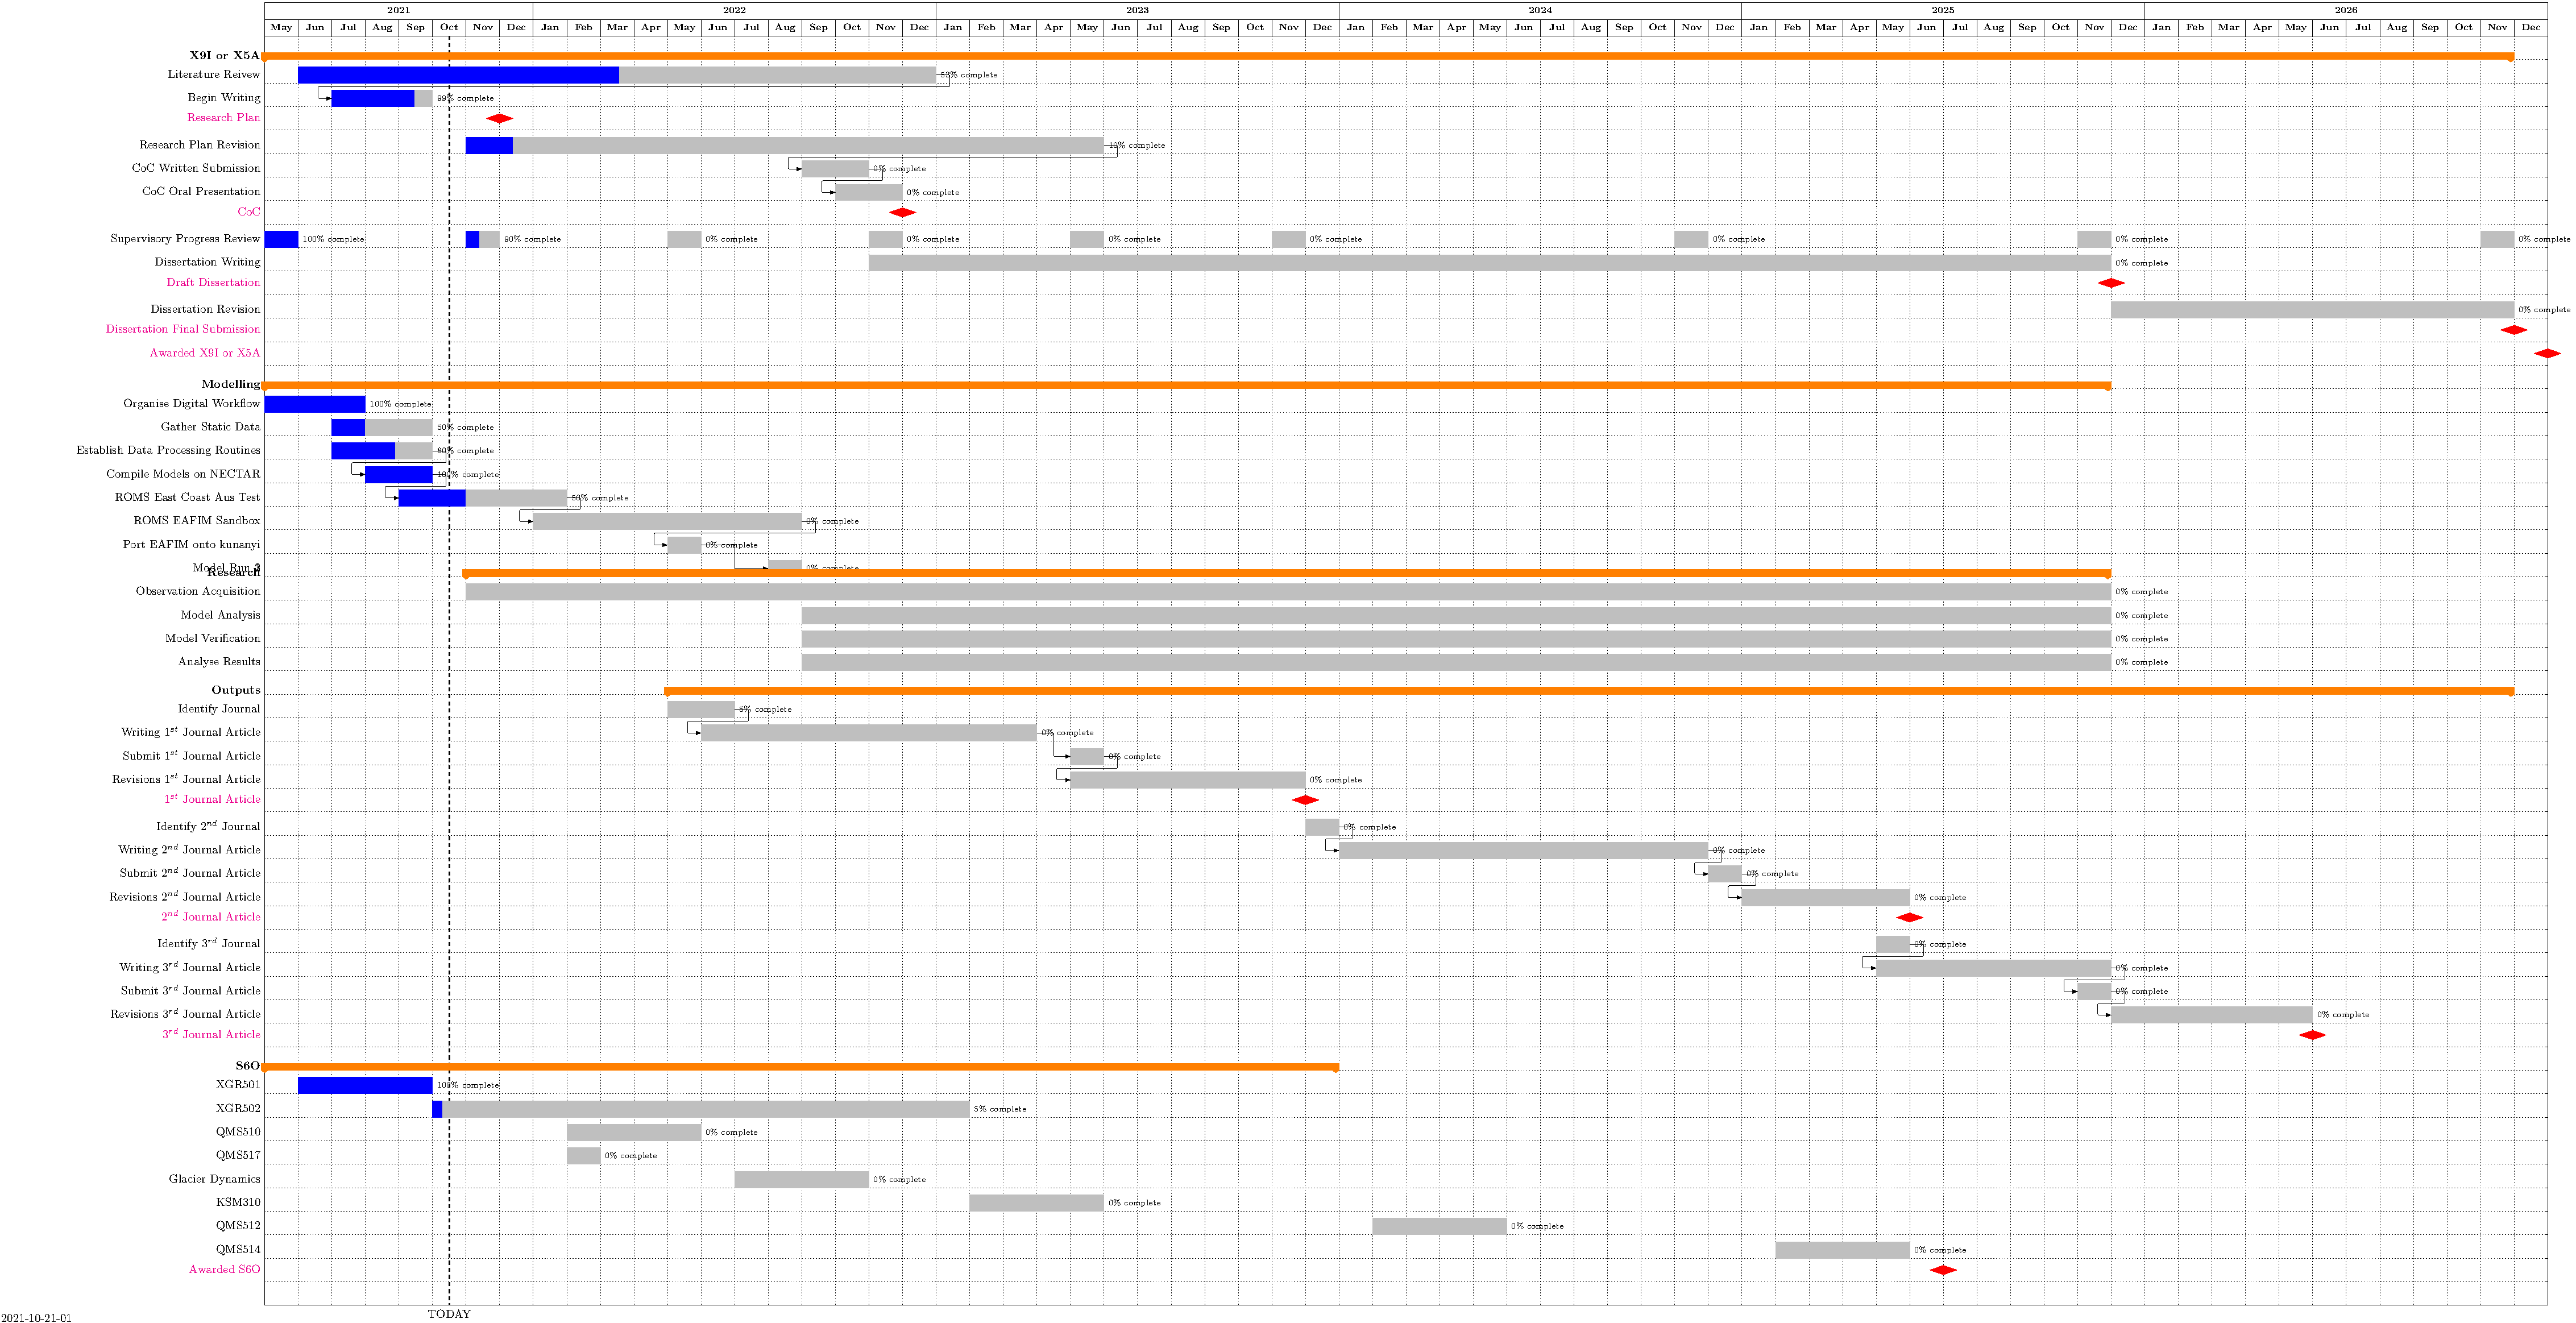
\includepdf[pages=-,pagecommand={},angle=90,width=.92\textwidth,height=.98\textheight]{ganttchart.pdf}
\end{landscape}
\restoregeometry
\newpage
%%%%%%%%%%%%%%%%%%%%%%%%%%%%%%%%%%%%%%%%
\section*{Budget}
\addcontentsline{toc}{section}{\protect\numberline{}Budget}%
\subsection{Scholarships}
\subsubsection{UTas RTP}
In receipt as part-time candidate. Essential.
\subsubsection{AAPP Top-Up}
Application withdrawn until employment level reduces to where this is required. Not essential.
\subsubsection{SCAR}
Applying for in 2022. Nice for international travel and collaboration.
\subsection{Travel}
\subsubsection{Remote to Hobart}
\subsubsection{Conferences}
\subsubsection{Collaborative}
\subsection{Infrastucture}
\subsubsection{Computing Hardware}
\begin{itemize}
\item Macbook Pro $\rightarrow$ paid for by IMAS
\item iPad
\end{itemize}
\subsubsection{Digital Subscriptions}
\begin{itemize}
\item Telstra
\item Terminus.app
\item GoodReader.app
\end{itemize}
\subsubsection{Professional Memberships}
\begin{itemize}
\item AMOS $\rightarrow$ student member
\item TOS $\rightarrow$ student member
\item AGU $\rightarrow$ student member
\item IGS $\rightarrow$ student member
\end{itemize}
%%%%%%%%%%%%%%%%%%%%%%%%%%%%%%%%%%%%%%%%
\section*{Ethical Approvals}
\addcontentsline{toc}{section}{\protect\numberline{}Ethical Approcals}%
Nil requirements.
%%%%%%%%%%%%%%%%%%%%%%%%%%%%%%%%%%%%%%%%
\section*{Work, Health and Safety}
\addcontentsline{toc}{section}{\protect\numberline{}WH\&S}%
Ergonomic risk assessment. Maintain good working posture and frequent breaks. Maintain good diet. Maintain a good exercise regime, at least 60 minutes of walking with body weight routine. Maintain sleep of at least 7 hours per night. Continue with meditation and music playing to relax and keep mentally fit.
%%%%%%%%%%%%%%%%%%%%%%%%%%%%%%%%%%%%%%%%
\section*{Intellectual Property}
\addcontentsline{toc}{section}{\protect\numberline{}IP}%
\doclicenseThis
%%%%%%%%%%%%%%%%%%%%%%%%%%%%%%%%%%%%%%%%
\section*{Project Infrastructure}
\addcontentsline{toc}{section}{\protect\numberline{}Project Infrastructure}%
\begin{itemize}
\item NECTAR
\item Cloudstor
\item kunanyi
\item Macbook Pro
  \begin{itemize}
  \item literature review
  \item writing
  \item email
  \item HPC communication
  \item visual meeting
  \item code development
  \end{itemize}
\item iPad
  \begin{itemize}
  \item literature review
  \item email
  \item HPC communication
  \end{itemize}
\end{itemize}
%%%%%%%%%%%%%%%%%%%%%%%%%%%%%%%%%%%%%%%%
\section*{Skills}
\label{sec:skills}
\addcontentsline{toc}{section}{\protect\numberline{}Skills}%
\begin{itemize}
\item Analytical Physics
\item Cryosphere Data Sampling
\item Satellite Remote Sensing
\item Geodectic Analysis
\item Numerical Modelling
\item Scientific Computer Programming
\item High Performance Computing
\item Scientific Writing
\item Scientific Presentation
\end{itemize}
%%%%%%%%%%%%%%%%%%%%%%%%%%%%%%%%%%%%%%%%
\section*{References}
\addcontentsline{toc}{section}{\protect\numberline{}References}%
\bibliography{../../references/refs.bib}
%%%%%%%%%%%%%%%%%%%%%%%%%%%%%%%%%%%%%%%%
\end{document}
}
%%%%%%%%%%%%%%%%%%%%%%
\end{document}
}
